% This is file JFM2esam.tex
% first release v1.0, 20th October 1996
%       release v1.01, 29th October 1996
%       release v1.1, 25th June 1997
%       release v2.0, 27th July 2004
%       release v3.0, 16th July 2014
%   (based on JFMsampl.tex v1.3 for LaTeX2.09)
% Copyright (C) 1996, 1997, 2014 Cambridge University Press

\documentclass{jfm}
\usepackage{graphicx}
\usepackage{epstopdf, epsfig}
\usepackage{amsmath}
\usepackage{amssymb}
\usepackage{wasysym}

\newtheorem{lemma}{Lemma}
\newtheorem{corollary}{Corollary}

\shorttitle{Role of forcing scale on $\beta$-plane turbulence}
\shortauthor{J. Chai and M. Jansen}

\title{Role of forcing scale on $\beta$-plane turbulence: jet formation}

\author{Junyi Chai\aff{1}
  \corresp{\email{junyi.x.chai@gmail.com}},
\and Malte Jansen\aff{2}}

\affiliation{\aff{1}Atmospheric and Oceanic Sciences Program, Princeton University, Princeton, New Jersey, USA
\aff{2}Department of the Geophysical Sciences, University of Chicago, Chicago, Illinois, USA}

\begin{document}

\maketitle

\begin{abstract}
Turbulence regimes are examined in forced-dissipative, two-dimensional
flow on a $\beta$-plane with emphasis on jet formation. 
The anisotropy of the flow is known to be largely determined
by the zonostrophic index $Z$, which is the ratio of the Rhines scale to
the turbulence-wave crossover scale. In this study, it is shown that the
forcing scale also influences the anisotropy, especially when it is 
comparable to or even larger than the crossover scale. The role of forcing scale
is characterized by a nondimensional number $\Pi$, which is the ratio of 
the classical crossover scale to the forcing scale.
Turbulence regimes are explored in $(Z,\Pi)$ space with numerical simulations. 
When $1.5\apprle Z\apprle2.5$, both $Z$ and $\Pi$ appear to influence jet formation: 
jets are stronger and easier to form for smaller $\Pi$. This behavior is understood
from a new form of crossover scale proposed for $\Pi<1$, which shows
that a wider range of scales is under $\beta$-effect than would be 
predicted from $Z$ alone. When $Z\apprge2.5$ and $\Pi\apprge4$, the flow is 
in the previously characterized zonostrophic turbulence regime, 
featuring strong jets. When $\Pi$ decreases, the jets become even sharper
and the flow gradually transits into a new turbulence regime at $\Pi\apprle1$. 
This regime is ``quasi-linear'' in the sense that eddy-eddy interactions
are negligible while eddy/mean-flow interactions dominate the nonlinear
energy and enstrophy transfers. The relevance of the quasi-linear regime
is discussed for the potential vorticity staircase limit, and 
for Earth's atmosphere and oceans.
\end{abstract}


\section{Introduction}

Planetary rotation profoundly affects the macroturbulence in the
atmosphere and ocean, distinguishing it from the flows at much smaller
scales in two different ways. First, the large scale flow is in near
geostrophic balance due to the rotation. Therefore macroturbulence
is quasi- two-dimensional in nature, which fundamentally changes the
picture for nonlinear energy transfer \citep{Kraichnan1967,Charney1971},
predictability \citep{Leith1971,Leith1972}, and tracer transport/mixing
\citep{Batchelor1959,Shuckburgh2003} from its three-dimensional counterpart.
Second, the differential rotation on a sphere, or $\beta$-effect,
introduces anisotropy to the flow. As a result, zonal jets spontaneously
form, and the flow becomes controlled by an interplay of turbulence, Rossby waves
and jets. Arguably, the simplest idealization to study the macroturbulence
with both effects of planetary rotation is a forced-dissipated two-dimensional
(2d) flow on a $\beta$-plane. This idealization contains the complexity
of nonlinear interactions, yet it is fully determined by a handful
of factors: forcing, dissipation (of both energy and enstrophy) and
$\beta$-effect. In this idealized setting, we can chart
different turbulent regimes using a few nondimensional numbers.
These turbulent regimes have their correspondence in the real geophysical
flows, as well as in models with increased complexity. Understanding
these regimes provide an important step towards a generalized theory 
of macroturbulent circulations on Earth and other planets.

One nondimensional number that is well-known to determine the anisotropy
of the flow is the ratio between two length scales: the Rhines scale
and the turbulence-wave crossover scale. The Rhines scale
can be viewed as the jet scale, and in terms of wavenumber it is
\begin{equation}
    k_{Rh}=(\beta/2U_{rms})^{1/2},\label{eq:Rhines_wavenumber_beta_Urms}
\end{equation}
where $U_{rms}$ is the rms velocity of the whole flow \citep{Rhines1975}.\footnote{
The form and meaning of Rhines scale have been
under debate since it has been proposed. In some studies, rms velocity
of the eddies or the meridional wind has been used, while the Rhines scale itself
has been used as an estimate for either eddy scale, jet scale, or
the scale where energy gets channeled into jets \citep{Williams1978,Jansen2012,Chai2014,Liu2015,Chemke2015}.
Here we choose the form and meaning that is most consistent 
with the theory of zonostrophic turbulence.}
The turbulence-wave crossover scale marks the transition from
isotropic eddies to Rossby waves, which in terms of wavenumber is
\begin{equation}
    k_{\varepsilon}=\mathcal{C}_{\varepsilon}\beta^{3/5}\varepsilon^{-1/5},\label{eq:classical_crossover_wavenumber}
\end{equation}
where $\varepsilon$ is the upscale energy flux and $\mathcal{C}_{\varepsilon}$ is a constant of about
$0.5\sim0.6$ \citep{Vallis1993,Galperin2010,Smith2002}. It is thought that
eddies smaller than the crossover scale are only weakly influenced by the 
$\beta$-effect, therefore behaving as isotropic turbulence, whereas eddies 
larger than the crossover scale predominately behave as Rossby waves.

Intuitively, the ratio of the two scales
\begin{equation}
    Z=k_{\varepsilon}/k_{Rh},\label{eq:zonostrophic_index_def}
\end{equation}
determines whether jets form or not, strong or weak, as the larger
$Z$ is, the larger range of scales of eddies become Rossby waves, whose
unique dispersion relation modifies their energy transfer in a way 
that most of the energy is directed into the zonal modes (a simple explanation 
is given by \citeauthor{Vallis1993}
{[}1993{]}; another explanation exploring a new invariant unique for
Rossby waves is given by \nocite{Balk1991,Balk2005}Balk {[}1991,
2005{]}, \citeauthor{Nazarenko2009} {[}2009{]}).
Specifically, \citet{Galperin2010}
divide $\beta$-plane turbulence into two regimes based on $Z$: 
\textit{zonostrophic} regime for $Z\gtrsim2.5$ and 
\textit{friction-dominated} regime for $Z\lesssim1.5$. 
Therefore, $Z$ is coined as the zonostrophic index. 
Zonostrophic turbulence gets its name because the flow
is dominated by strong zonal jets. The friction-dominated
regime is close to isotropic turbulence as the inverse energy cascade
is halted by friction before reaching the crossover scale.

Quantitatively, the energy spectra of eddies (defined here as deviations
from the zonal mean) and zonal flow for zonostrophic turbulence, as 
illustrated in Fig. \ref{EKE_KE_spectra_illustrate}, further
explain how the zonostrophic index $Z$ sets the anisotropy of the flow. 
Let the 2d flow be stirred by a spectrally localized forcing at a (high) wavenumber $k_{f}$.
The eddies have the same energy spectrum as in isotropic turbulence,
with an inverse energy cascade range for $k<k_f$ where
\begin{equation}
    \mathcal{E}(k)=\mathcal{C}_K\varepsilon^{2/3}k^{-5/3},\label{eq:Kolmogorov_Kraichnan_spectrum_energy}
\end{equation}
and a steeper direct enstrophy cascade range for $k>k_f$, where
\begin{equation}
    \mathcal{E}(k)=\mathcal{C'}_K\eta^{2/3}k^{-3}.\label{eq:Kolmogorov_Kraichnan_spectrum_enstrophy}
\end{equation}
Here $\varepsilon$ and $\eta$ are the upscale energy and downscale enstrophy
fluxes respectively; $\mathcal{C}_K$ and $\mathcal{C'}_K$ 
are the Kolmogorov constants of about $6\sim7$ and $1.3\sim1.6$ respectively
\citep{Maltrud1991,Smith1993,Paret1997,Chen2006,Borue1993,Gotoh1998}.
The central piece of zonostrophic turbulence is that 
energy in the zonal modes (jets) follows a universal spectrum determined
by $\beta$ and wavenumber as
\begin{equation}
\mathcal{E}_{Z}(k)=\mathcal{C}_Z\beta^{2}k^{-5},\ k_{x}=0,\label{eq:zonostrophic_spectrum}
\end{equation}
where $k_{x}$ is the zonal wavenumber, and the constant $\mathcal{C}_Z$
is uncertain but roughly about 0.2$\sim$0.5 \citep{Sukoriansky2002,Galperin2010,Smith2005}.
Indications for such spectrum have been observed in many numerical simulations 
\citep{Chekhlov1996,Smith2002,Huang2001,Sukoriansky2002,Sukoriansky2007},
in the Jovian atmosphere \citep{Sukoriansky2002,Choi2011,Galperin2014}
and even in high-resolution ocean simulations \citep{Galperin2004}.
Zonal and eddy energy spectra intersect at the crossover wavenumber $k_{\varepsilon}$.
Eventually, friction comes into effect and halts the energy 
cascade at the jet scale $k_r^{-1}$,
which is related to the Rhines scale as mentioned before.\footnote{
The zonal spectrum (\ref{eq:zonostrophic_spectrum})
also lays Rhines scale on a quantitative ground: assuming
that most energy is in the jets, an integration of (\ref{eq:zonostrophic_spectrum}) 
from $k_{r}$ to $\infty$ gives total energy as $\mathcal{C}_Z\beta^{2}k_{r}^{-4}/4$,
and then using $\mathcal{C}_Z\sim 0.5$ and (\ref{eq:Rhines_wavenumber_beta_Urms})
we can get $k_{r}\simeq k_{Rh}$.}
As the zonal energy spectrum (\ref{eq:zonostrophic_spectrum}) 
contains much more energy than the eddy energy spectrum 
(\ref{eq:Kolmogorov_Kraichnan_spectrum_energy}) for $k<k_\varepsilon$,
jets dominate the flow when $Z$ is large.

The above zonostrophic turbulence picture and the derivation of
the crossover scale in (\ref{eq:classical_crossover_wavenumber}) assume
that the forcing scale is much smaller than the crossover scale so that
there exists an extended inverse cascade range in between.
The details of the forcing, including the forcing scale,
may lose their influence on the large scale flow due to
the locality hypothesis. This is probably true when $k_{f}/k_{\varepsilon}\apprge4$,
which is noted by \citet{Sukoriansky2007} as a prerequisite
to reach zonostrophic turbulence and can be understood from the fact
that the inverse cascade is only weakly local in scale: 
energy flux across scale $l$ involves
the thinning of subscale eddies 4 to 8 times smaller than $l$ by
the strain at $l$ \citep{Chen2006}.
The condition $k_{f}/k_{\varepsilon}\apprge4$, however, 
is not satisfied in Earth's atmosphere \citep{Schneider2006,Merlis2009}
and oceans \citep{Tulloch2011}. In this case, the details of
forcing may not be negligible. Furthermore, literature 
on potential vorticity (PV) staircases hints at the fact that
the forcing scale itself can play an important role 
in jet formation especially when it is comparable to the crossover scale \citep{Scott2012}.
The PV staircase has long been hypothesized as a model for jet formation.
In its ideal limit, the PV staircase implies that PV is
perfectly mixed between jets while having distinct jumps at the center
of jets \citep{Marcus1993,Marcus1998,Dunkerton2008,Dritschel2008}.
A flow with a near-perfect PV staircase structure has been 
simulated by \citet{Scott2012}, who suggest the very high
zonostrophic index as the key to obtain the PV staircase. 
Although dominated by strong jets in zonostrophic turbulence,
a perfect PV staircase has a shallower spectral slope than
(\ref{eq:zonostrophic_spectrum}) as follows directly from the
relationship between the PV and flow field \citep{Saffman1971,Danilov2004}.
This suggests that the PV staircase may not represent the zonostrophic
regime despite having very high zonostrophic index. In fact,
examining the setup of \citet{Scott2012} suggests that 
$k_{f}/k_{\varepsilon}<1$, indicating that a relative large forcing
scale may be an additional requirement to reach the PV staircase regime.\footnote{
In a later study, \citet{Scott2012a} suggest that PV staircase can
easily form when the forcing scale is as large as the jet scale and
$k_{f}/k_{\varepsilon}\apprle1/6$, which is more extreme than the
condition we suggest here. This extreme regime is reached by a rather
unusual topographic forcing without large scale friction, which makes
it not straightforward to compare with the forced-dissipative turbulence
in this study.} 

In this study, we aim to answer how the forcing scale influences the
flow. From the above discussion, the ratio
\begin{equation}
\Pi=k_{f}/k_{\varepsilon}\label{eq:def_Pi_index}
\end{equation}
suggests itself as an important nondimensional number to characterize
the role of the forcing scale. When $\Pi<1$, the crossover scale $k_{\varepsilon}^{-1}$
is now within the direct enstrophy cascade range and therefore the formulation
of the turbulence-wave crossover scale in (\ref{eq:classical_crossover_wavenumber})
should no longer hold. 

This paper is organized
as follow. In section 2, we derive a new crossover scale in the
enstrophy cascade branch for $\Pi<1$. In section 3, a set of experiments
varying both $\Pi$ and $Z$ are carried out. Experiment results are
analyzed in section 4 using turbulent phenomenology
and our new crossover scale. In section 5, we conclude with an updated
chart for turbulence regimes in ($Z$, $\Pi$) space and discuss
its relevance for observed geophysical flows.


\section{Theory}

In this section, we follow the derivation of \citet{Vallis1993} for
the classical turbulence-wave crossover scale but generalize it
for the case $\Pi<1$. First consider scalings in a 2d flow forced
at wavenumber $k_{f}$ based on the phenomenology of isotropic turbulence. 
Energy inversely cascades to larger scales and
enstrophy directly cascades to smaller scales. The inverse of the eddy
turnover time defines a strain rate, or ``turbulence frequency''
$\omega_{t}$. From dimensional analysis, the turbulence frequency in 
the inverse energy cascade branch ($k<k_f$) is
\begin{equation}
\omega_{t}=\mathcal{C}_{\omega,\varepsilon}\varepsilon^{1/3}k^{2/3},\label{eq:eddy_turnover_freq_inverse_cascade}
\end{equation}
and in the direct enstrophy cascade branch ($k>k_f$) is
\begin{equation}
\omega_{t}=\mathcal{C}_{\omega,\eta}\eta^{1/3},\label{eq:eddy_turnover_freq_direct_enstrophy_cascade}
\end{equation}
where $\mathcal{C}_{\omega,\varepsilon}$ and $\mathcal{C}_{\omega,\eta}$
are nondimensional universal constants. If the forcing scale is 
well localized, the enstrophy flux is related to the energy flux by
\begin{equation}
\eta=k_{f}^{2}\varepsilon.\label{eq:energy_enstrophy_flux_relationship}
\end{equation}
As $\omega_{e}$ must be continuous across $k_{f}$, we have
\begin{equation}
\mathcal{C}_{\omega,\varepsilon}\varepsilon^{1/3}k_{f}^{2/3}=\mathcal{C}_{\omega,\eta}\eta^{1/3}.\label{eq:turbulence_freq_continuity}
\end{equation}
Using the relations (\ref{eq:energy_enstrophy_flux_relationship}) and (\ref{eq:turbulence_freq_continuity}),
we relate the two constants as $\mathcal{C}_{\omega,\varepsilon}=\mathcal{C}_{\omega,\eta}$.
Therefore, $\omega_{t}$ can be written concisely as
\begin{equation}
\omega_{t}=\mathcal{C}_{\omega,\varepsilon}\varepsilon^{1/3}\begin{cases}
k^{2/3}, & k<k_{f}\\
k_{f}^{2/3}, & k>k_{f}
\end{cases},\label{eq:eddy_turnover_freq_general_form}
\end{equation}
which is a monotonic nondecreasing function with $k$.

The Rossby wave frequency is 
\begin{equation}
\omega_{\beta}=-\frac{\beta k_{x}}{k^{2}}.\label{eq:Rossby_wave_freq_kx_k}
\end{equation}
As the crossover scale is at the isotropic turbulence boundary, we
take $k_{x}\sim k$ and get the magnitude of the Rossby wave frequency as
\begin{equation}
|\omega_{\beta}|\simeq\frac{\beta}{k}.\label{eq:Rossby_wave_freq_k}
\end{equation}
As illustrated in Fig. \ref{crossover_illustrate}, the turbulence frequency
$\omega_{t}$ and Rossby wave frequency $|\omega_{\beta}|$ intersects at a
unique wavenumber -- the turbulence-wave crossover wavenumber.
If $\Pi>1$, the crossover scale is within the energy cascade range as
$|\omega_\beta|$ intersects with the energy cascade branch of $\omega_t$,
which gives the classical scaling $k_\varepsilon$ in (\ref{eq:classical_crossover_wavenumber}).
If $\Pi<1$, the crossover scale is now within the enstrophy cascade regime
as $|\omega_\beta|$ intersects with the enstrophy cascade branch of $\omega_t$
at 
\begin{equation}
k_{\eta}=\mathcal{C}_{\omega,\varepsilon}^{-1}\beta\varepsilon^{-1/3}k_{f}^{-2/3}.\label{eq:crossover_k_enstrophy_branch}
\end{equation}
In this case the classical crossover wavenumber $k_\varepsilon$ loses its meaning.
However, for convenience of use, we can rewrite this new crossover wavenumber $k_\eta$
in terms of $k_\varepsilon$ and $\Pi$ as
\begin{equation}
k_{\eta}=\Pi^{-2/3}k_{\varepsilon}.\label{eq:k_eta_k_epsilon_relation}
\end{equation}
The generalized crossover wavenumber can thus be summarized as
\begin{equation}
k_{\beta}=\max(k_{\varepsilon},k_{\eta})=k_{\varepsilon}\max(1,\Pi^{-2/3}),\label{eq:generalized_crossover_wavenumber}
\end{equation}
where $\max(x,y)$ returns the larger of $x$ and $y$. 

The range of scales influenced by the $\beta$-effect determines
how anisotropic the flow is. When $\Pi<1$, 
$k_{\varepsilon}$ underestimates the generalized crossover wavenumber.
In this case, the zonostrophic index $Z$ underestimates the range
of scales influenced by the $\beta$-effect and thus should underestimate the anisotropy
of the flow. Using the generalized crossover wavenumber $k_{\beta}$,
we may define a ``jet index'' to properly measure the width of the
range of scales influenced by the $\beta$-effect as
\begin{equation}
Z_{J}=\frac{k_{\beta}}{k_{Rh}}=\max(1,\Pi^{-2/3})Z.\label{eq:jet index}
\end{equation}
Here we assume that the Rhines scale still roughly gives the energy
halting scale, though the energy halting scale will probably have a
dependency on $\Pi$ as the universal spectrum (\ref{eq:zonostrophic_spectrum})
is unlikely to hold in the $\Pi<1$ regime as discussed in the introduction. 
Using the jet index, we would
expect the jets to be even stronger if $\Pi$ is reduced to below 1 for
the same zonostrophic index. It could also mean that jet 
formation may be easier when $\Pi$ is reduced
below 1 for the same zonostrophic index $Z$: the boundary of jet
formation is determined by both $Z$ and $\Pi$. 

A caveat in the above derivation is that the turbulence frequency (\ref{eq:eddy_turnover_freq_direct_enstrophy_cascade})
is in the form of isotropic turbulence. However, when $\Pi<1$
the forcing scale is larger than the crossover scale
so we cannot expect eddies at the forcing scale to be isotropic
turbulence as they already behave as Rossy waves.
The derivation is rescued by noting that the enstrophy cascade is expected
to be non-local. The dominant straining at $k>k_{f}$ comes from
the shear of the largest scale jets. The eddies are sheared apart
by the jets and thus transfer enstrophy directly to much smaller scales.
The turbulence frequency should now be interpreted as the eddy
decorrelation rate, which scales with the shear of the jets and therefore
is independent of $k$. So the form of $\omega_{t}$ in (\ref{eq:eddy_turnover_freq_direct_enstrophy_cascade})
is retained and so is the rest of the derivation. The non-local enstrophy
cascade dominated by eddy/mean-flow interactions is seen in previous
studies \citep{Manz2009} and also in our simulations (Section 4).
Even in pure isotropic 2d turbulence, some studies suggest that the enstrophy
cascade is perhaps highly non-local, and the process is close to the cascade
of a passive tracer \citep{Borue1993,Falkovich1994}.


\section{Model description and experiments}

Forced-dissipated 2d flow on a $\beta$-plane described as

\begin{equation}
\frac{\partial\zeta}{\partial t}+J(\psi,\zeta)+\beta v=\vartheta-\nu\nabla^{8}\zeta-r\zeta\label{eq:barotropic_vorticity_eq}
\end{equation}
is solved on a doubly-periodic $2\pi\times2\pi$ square domain. On
the left hand side, $\psi$ is the stream function, $v=\partial\psi/\partial x$
is the meridional velocity, $\zeta=\nabla^{2}\psi$ is the relative vorticity,
and $\beta$ is the planetary vorticity gradient. On the right hand
side, $\vartheta$ represents the forcing, while the dissipation consists
of a linear friction $-r\zeta$ and an 8th order hyperviscosity dissipation
$-\nu\nabla^{8}\zeta$. The hyperviscosity $\nu$ is adjusted adaptively
in the numerical model using an optimal estimate similar to a 
Smagorinsky viscosity (see details in \citeauthor{Maltrud1991}
{[}1991{]} and \citeauthor{Smith2002} {[}2002{]}). 
The forcing $\vartheta$ is defined
in spectral space via its Fourier transform $\{\vartheta\}_{k}$,
which has a uniform distribution within a narrow band $[k_{f}-\delta k_{f},k_{f}+\delta k_{f}]$.
The half width of the spectrum band is $\delta k_{f}=2$ in all our
simulations. In time, $\{\vartheta\}_{k}$ is random Markovian with
a very short decorrelation time (correlation falls under 5\% after
5 time steps) and normalized at each time step so that the energy
injection rate
\begin{equation}
\varepsilon_{0}=-\langle\psi\vartheta\rangle\label{eq:energy_injection_rate}
\end{equation}
is fixed at a prescribed level, which is very close to the upscale
energy flux $\varepsilon$ when the forcing scale is far away from grid
scale. The angle bracket $\langle*\rangle$ denotes domain averaging.
Numerical integration is performed using a de-aliased pseudo-spectral
method for space differentiating with a maximum resolved wavenumber
of 511 (1024$^{2}$ equivalent horizontal gridpoints), and a leap-frog
method with a weak Robert filter for time stepping \citep{Patterson1971}.
More details on the model are described in \citet{Smith2002}.

Ignoring the dependency on the exact form of the random forcing 
($\delta k_f$, decorrelation time scale, etc.), Eq. (\ref{eq:barotropic_vorticity_eq})
is fully characterized by 4 nondimensional
numbers constructed from \{$\varepsilon$,$\beta$,$r$,$k_{f}$,$L$,$\nu$\},
where $L$ is the size of the domain. If we assume that the energy has
not reached the domain size so that $L$ does not matter, and that the
enstrophy is dissipated at a small enough scale so that hyperviscosity
$\nu$, which determines the exact scale of enstrophy dissipation,
does not matter, the system is fully characterized
by 2 nondimensional numbers constructed from \{$\varepsilon$,$\beta$,$r$,$k_{f}$\}.
As mentioned in the introduction, the two nondimensional numbers
are chosen to be the zonostrophic index 
\[
Z=k_{\varepsilon}/k_{Rh},
\]
and
\[
\Pi=k_{f}/k_{\varepsilon}.
\]
Multiplying (\ref{eq:barotropic_vorticity_eq}) with $-\psi$ yields
an equation governing the time evolution of energy $E$ as
\begin{equation}
\frac{dE}{dt}=\varepsilon-2rE.\label{eq:energy_evolution_equation}
\end{equation}
In equilibrium, the domain averaged total kinetic energy $E$ and
thus rms velocity $U_{rms}$ can be related to the upscale energy flux
and frictional rate $r$ as
\[
2rE=\varepsilon,
\]
where 
\[
E=\frac{1}{2}\langle u^{2}+v^{2}\rangle=\frac{1}{2}U_{rms}^{2}.
\]
The Rhines wavenumber in (\ref{eq:Rhines_wavenumber_beta_Urms}) can thus
be rewritten as
\begin{equation}
k_{Rh}=2^{-1/2}\beta^{1/2}r^{1/4}\varepsilon^{-1/4}.\label{eq:Rhines_wavenumber_beta_r_epsilon}
\end{equation}
Using Eqs. (\ref{eq:classical_crossover_wavenumber}), (\ref{eq:zonostrophic_index_def}), 
(\ref{eq:def_Pi_index}) and (\ref{eq:Rhines_wavenumber_beta_r_epsilon}) we can express $Z$ and $\Pi$ as
\begin{equation}
Z=0.85\beta^{1/10}\varepsilon^{1/20}r^{-1/4},\label{eq:Z_estimate_in_work}
\end{equation}
and
\begin{equation}
\Pi=1.67\beta^{-3/5}\varepsilon^{1/5}k_{f},\label{eq:PI_estimate_in_work}
\end{equation}
where we use $\mathcal{\mathcal{C}_{\varepsilon}}=0.6$ in (\ref{eq:classical_crossover_wavenumber}).

As $Z$ and $\Pi$ have the highest power law dependency on $r$ and
$k_{f}$ respectively, it is easiest to vary $r$ and $k_{f}$ to
explore the $(Z,\Pi)$ space. In order to make sure that the energy cascade is
always halted before reaching the domain size when we vary $r$, we impose
the ratio $\varepsilon_{0}/r$=$(\pi/4)^{2}$ and $\beta=16\pi$ so
that $k_{Rh}\simeq5.7$, as used by \citet{Scott2012}. In
the actual simulations, the number of jets varies from 3 to 5, which
largely agrees with the Rhines wavenumber. The linear friction rate
$r$ is varied among $10^{-4}\times$(4096, 1024, 256, 64, 8, 1) so
that the zonostrophic index $Z$ varies from 1.4 to 7.3. For each frictional
rate $r$, forcing wavenumber $k_{f}$ is varied among 16, 32, 64
and 128 (for the lowest friction $r=10^{-4}$, one experiment $k_{f}=128$
is not carried out due to the high computational cost to simulate
such a low-friction flow). A consideration
on the choice of forcing scale is that the forcing scale should be
smaller than the energy halting scale. Otherwise the flow is
uninteresting as energy is directly dissipated by friction at the
forcing scale without much nonlinear interactions.
The largest forcing scale here ($k_{f}=16$) is
still sufficiently smaller than the jet scale so that we ensure
enough room for nonlinear interactions. Under the above consideration,
we can draw a crude boundary in the $(Z,\Pi)$ space
for the flow to be interesting:
\begin{equation}
\Pi Z=k_{f}/k_{Rh}>1.\label{eq:PIxZ>1}
\end{equation}
The $(Z,\Pi)$ space that is explored is shown in Fig. \ref{anisotropic_index},
where each simulation is indicated by either a dot or a triangle. The
regime $\Pi<1$ is reached in some simulations with relatively large
zonostrophic index $Z\apprge3$. 

Theoretically, we can sample the corner of $(Z,\Pi)$ space where
both $Z$ and $\Pi$ are high by simply increasing the forcing wavenumber.
In reality, however, this would require a prohibitive computational
power. The high $Z$ regime needs a long time to equilibrate, which
roughly scales as $1/r$. In practice, the flow with the
highest $Z=7.3$ requires computational time 4 to 5 orders of magnitudes
higher than the flow with $Z=1.4$. Further increasing $\Pi$ by increasing
forcing wavenumber for the $Z=7.3$ run requires increasing horizontal
resolution as well, which again becomes computationally prohibitive with
our current resources.


\section{Results}

In the zonostrophic turbulence picture, the anisotropy of the flow is
determined by the zonostrophic index $Z$, and the flow regime is
divided into friction-dominated ($Z\apprle1.5$), transitional ($1.5\apprle Z\apprle2.5$)
and zonostrophic ($Z\apprge2.5$). In this section, we look at the
influence of $\Pi$ on the flow when the zonostrophic index $Z$ is
relatively small ($Z\apprle2.5$) or large ($Z\apprge2.5$). Finally,
the formation of PV staircase when $Z$ is very large ($Z\apprge7.3$)
is examined.

\subsection*{a. Jet formation boundary ($Z\apprle2.5$)}

As a metric for the anisotropy (or jet strength)
in the $(Z,\Pi)$ space, we define an anisotropy index $\chi$ as
\begin{equation}
\chi=\langle\frac{u^{2}}{u^{2}+v^{2}}\rangle,
\end{equation}
which measures the percentage of energy in the zonal wind. For
isotropic turbulence, the anisotropy index $\chi$ should be 0.5
as there is no difference between $u$ and $v$. In the $(Z,\Pi)$
space, the anisotropy index is shown in Fig. \ref{anisotropic_index}.
Black dots indicate that jets have formed in the corresponding run,
whereas gray triangles indicate that there is no visually identifiable
jet in that run. Across the whole parameter space here, $Z$ is the
dominant factor that shapes the overall behavior of the anisotropic
index: $\chi$ increases monotonically from about 0.5 to near 1 when
$Z$ increases from about 1.4 to 7.3. For the lowest $Z=1.4$, $\chi\approx0.5$
confirms the flow to be in the friction-dominated regime as would
be predicted by the criterion $Z\apprle1.5$. Indeed, no jet or even
slight hint of jet is seen in any of the $Z=1.4$ runs. Anisotropy of the flow 
seems not to be dependent on $\Pi$ in the range we 
explored as seen from $\chi$ here.

Jets start to form when $Z\apprge1.8$. For the two series of runs
$Z=1.8$ and 2.4 within the transitional regime $1.5\apprle Z\apprle2.5$,
$\Pi$ clearly influences the anisotropy of the flow with $\chi$ increasing
as $\Pi$ decreases. The influence of $\Pi$ on the formation and
strength of the jet is seen more intuitively from the vorticity and zonal
velocity fields shown in Fig. \ref{vor_u_snapshot_drag1024e-4} (for
$Z=1.8$) and \ref{vor_u_snapshot_drag256e-4} (for $Z=2.4$). Arguably,
among the $Z=1.8$ runs, visually identifiable jets are only seen in the
run with the smallest $\Pi=1.5$. Though whether jets have formed
or not in this run is subjective, it is clear that the flow with $\Pi=1.5$
is much more anisotropic than the one with $\Pi=11.9$ (comparing
Fig. \ref{vor_u_snapshot_drag1024e-4} top with bottom). For the larger
$Z=2.4$, jets form in all runs (up to some debate for the run with
$\Pi=9.0$), but are stronger and more coherent when $\Pi$ is
smaller. Therefore, we conclude that not only the zonostrophic index
$Z$ but also $\Pi$ determines the boundary for jet formation, as
well as the coherence and strength of the jets. This dependency on
$\Pi$ qualitatively agrees with our theory, which predicts that the
jet index $Z_{J}$ -- as an indicator of jet strength -- increases
when $\Pi$ decreases. Quantitatively however, our theory predicts that
such a dependency only exists when $\Pi<1$. In the simulations, the
influence of $\Pi$ extends to a much greater extent than $\Pi<1$.
Nevertheless, it is clear that the influence is stronger
when $\Pi$ is closer to 1, and $\Pi$ gradually loses importance
when it becomes larger than 4 (as seen in inset of Fig. \ref{anisotropic_index}
and by visually examining the flows).
The observed larger extent of influence than $\Pi<1$ is hardly a
surprise. As we mentioned in the introduction, the inverse energy cascade
must at least extend to 4 times of the forcing scale in order for
the forcing scale to lose its influence \citep{Chen2006}. Therefore,
we expect $\Pi$ to influence jet formation as far as $\Pi\apprle4$
but to gradually lose importance when $\Pi$ increases above $\sim 4$.


\subsection*{b. From zonostrophic to ``quasi-linear'' turbulence ($Z\apprge2.5$)}

The condition for zonostrophic turbulence is that $Z\apprge2.5$ and $\Pi\apprge4$
\citep{Sukoriansky2007,Galperin2010}. In our simulations with $Z=4.8$,
$\Pi$ varies from about 0.6 to 4.5. As seen from vorticity and zonal
wind fields in Fig. \ref{vor_u_snapshot_drag8e-4}, the jets are
strong for all values of $\Pi$. Still, for smaller $\Pi\apprle 1$,
the jets are even sharper and more coherent than those in the zonostrophic turbulence
regime with $\Pi=4.5$, qualitatively consistent with the prediction
that the jet index $Z_{J}$ is increased for small $\Pi$. 
More importantly, when $\Pi<1$ the generalized crossover
scale $k_{\beta}^{-1}$ is smaller than the forcing scale so we may expect
$\Pi<1$ to be in a new turbulence regime with a qualitative different
energy cascade than the zonostrophic regime. In the following, we
focus on characterizing and understanding this regime in spectral space.

The kinetic energy spectrum can be evaluated as
\begin{equation}
\mathcal{E}(k)=\frac{1}{2}\underset{|\mathbf{k}|=k}{\sum}k^{2}|\left\{ \psi\right\} _{\mathbf{k}}|^{2}=-\frac{1}{2}\underset{|\mathbf{k}|=k}{\sum}\left\{ \zeta\right\} _{\mathbf{k}}\left\{ \psi\right\} _{\mathbf{k}}^{*},\label{eq:energy_spectrum_psi_zeta}
\end{equation}
where the bracket $\left\{ A\right\} _{\mathbf{k}}$ denotes the Fourier
component of $A$ at wave vector $\mathbf{k}=(k_{x},k_{y})$, the
star $A^{*}$ denotes complex conjugate of $A$. The spectrum $\mathcal{E}(k)$
can be decomposed into a sum of the eddy kinetic energy (EKE) spectrum
\begin{equation}
\mathcal{E}_{eddy}(k)=\frac{1}{2}\underset{|\mathbf{k}|=k,k_{x}\neq0}{\sum}k^{2}|\left\{ \psi\right\} _{\mathbf{k}}|^{2},\label{eq:EKE_spec_psi}
\end{equation}
and the zonal kinetic energy (ZKE) spectrum
\begin{equation}
\mathcal{E}_{Z}(k)=\frac{1}{2}\underset{|\mathbf{k}|=k,k_{x}=0}{\sum}k^{2}|\left\{ \psi\right\} _{\mathbf{k}}|^{2}.\label{eq:ZKE_spec_psi}
\end{equation}
The energy spectra of the total flow $\mathcal{E}(k)$, of the eddies
$\mathcal{E}_{eddy}(k)$ and of the zonal flow $\mathcal{E}_{Z}(k)$
are shown in Fig. \ref{E_EKE_ZKE_spectrum_drag8e-4}. The theoretical
spectra from the zonostrophic turbulence picture for the inverse energy 
cascade range (\ref{eq:Kolmogorov_Kraichnan_spectrum_energy}),
the enstrophy cascade range (\ref{eq:Kolmogorov_Kraichnan_spectrum_enstrophy}),
and the zonal modes (\ref{eq:zonostrophic_spectrum}) 
are shown for a comparison. The universal constants are chosen as
$\mathcal{C}_{K}=6$, $\mathcal{C'}_{K}=1.6$ and $\mathcal{C}_{Z}=0.5$
as those reported in the literature \citep{Boffetta2012,Galperin2010}.

For the runs with $\Pi=4.5$ and 2.3, the energy spectra show some
resemblance with the zonostrophic turbulence picture illustrated in 
Fig. \ref{EKE_KE_spectra_illustrate}: (a) the EKE spectrum $\mathcal{E}_{eddy}(k)$ 
roughly follows the theoretical isotropic inverse cascade spectrum 
(\ref{eq:Kolmogorov_Kraichnan_spectrum_energy}) with -5/3 slope
from the forcing scale all the way to slightly less than the energy
halting scale, and (b) the ZKE spectrum $\mathcal{E}_{Z}(k)$
is much steeper than $\mathcal{E}_{eddy}(k)$ and is roughly consistent with a -5 slope
between the crossover scale and the energy halting scale. However, the theoretical
universal spectrum (\ref{eq:zonostrophic_spectrum}) overestimates 
the energy level of $\mathcal{E}_{Z}(k)$, which results in the zonal
and eddy spectra to intersect at a scale larger than the predicted
crossover scale. Notice that for the runs here, the slope of ZKE spectrum
cannot be measured very accurately because there are only a couple of 
jets in the runs.

When $\Pi$ decreases below 1 to $\Pi=0.6$, two significant changes are 
visible in the spectra. First, the classical inverse cascade spectrum 
with $-5/3$ slope disappears but the EKE spectrum follows $-3$ slope 
in both the inverse cascade branch ($k<k_{f}$) and the  enstrophy cascade branch ($k>k_{f}$). Second, the scale where the total spectrum $\mathcal{E}(k)$ starts to
steepen above the EKE spectrum moves from scales larger than the forcing scale to
smaller than the forcing scale, while staying roughly close to the generalized
crossover scale ($k_\varepsilon$ or $k_\eta$ in Fig. \ref{E_EKE_ZKE_spectrum_drag8e-4}).
This is consistent with the expectation that the crossover scale 
becomes smaller than forcing scale when $\Pi<1$. 

For $\Pi<1$, the flow lacks the classic inverse cascade range as 
suggested by the absence of a $-5/3$ EKE spectrum slope. Instead, eddies at 
the forcing scale are already influenced by the $\beta$-effect. What effect 
does this have on the energy cascade? To gain more insight, 
we resort to the spectral energy budget, 
which is obtained by multiplying $-\widetilde{\psi}_{\mathbf{k}}^{*}$
to the Fourier transform of the vorticity equation (\ref{eq:barotropic_vorticity_eq})
and then using the form of the energy spectrum in (\ref{eq:energy_spectrum_psi_zeta}).
The spectral energy budget is
\begin{equation}
\frac{\partial\mathcal{E}(k)}{\partial t}=T(k)-\underset{|\mathbf{k}|=k}{\sum}\left\{ \psi\right\} _{\mathbf{k}}^{*}\left\{ \vartheta\right\} _{\mathbf{k}}-2r\mathcal{E}(k),\label{eq:spectral_energy_budget}
\end{equation}
where we neglect energy dissipation by hyperviscosity. The term $T(k)$
is the nonlinear energy transfer into wavenumber $k$:
\begin{equation}
T(k)=\underset{|\mathbf{k}|=k}{\sum}\left\{ \psi\right\} _{\mathbf{k}}^{*}\left\{ J(\psi,\zeta)\right\} _{\mathbf{k}}.
\end{equation}
The other terms $-\Sigma_{|\mathbf{k}|=k}\left\{ \psi\right\} _{\mathbf{k}}^{*}\left\{ \vartheta\right\} _{\mathbf{k}}$
and $-2r\mathcal{E}(k)$ are forcing and dissipation, respectively.
We can further decompose the flow into a sum of the eddy and zonal-mean contributions as
\begin{equation}
\psi=\overline{\psi}+\psi',
\end{equation}
where $\overline{A}$ denotes the zonal mean of $A$, and 
$A'$ denotes the deviation from the zonal mean. The spectral EKE
budget can then be formulated as
\begin{equation}
\frac{\partial\mathcal{E}_{eddy}(k)}{\partial t}=T_{EE}(k)-T_{EM}^{e}(k)-\underset{|\mathbf{k}|=k}{\sum}\left\{ \psi'\right\} _{\mathbf{k}}^{*}\left\{ \vartheta'\right\} _{\mathbf{k}}-2r\mathcal{E}_{eddy}(k),\label{eq:spectral_EKE_budget}
\end{equation}
where the eddy-eddy interaction is 
\begin{equation}
T_{EE}(k)=\underset{|\mathbf{k}|=k}{\sum}\left\{ \psi'\right\} _{\mathbf{k}}^{*}\left\{ J(\psi',\zeta')\right\} _{\mathbf{k}},
\end{equation}
and the eddy/mean-flow interaction is
\begin{equation}
T_{EM}^{e}(k)=-\underset{|\mathbf{k}|=k}{\sum}\left\{ \psi'\right\} _{\mathbf{k}}^{*}\left\{ \overline{u}\frac{\partial\zeta'}{\partial x}+v'\frac{\partial\overline{\zeta}}{\partial y}\right\} _{\mathbf{k}}.
\end{equation}
The spectral ZKE budget is
\begin{equation}
\frac{\partial\mathcal{E}_{\mathcal{Z}}(k)}{\partial t}=T_{EM}^{m}(k)-2r\mathcal{E}_{\mathcal{Z}}(k),\label{eq:spectral_ZKE_budget}
\end{equation}
where the eddy/mean-flow interaction is
\begin{equation}
T_{EM}^{m}(k)=\underset{|\mathbf{k}|=k}{\sum}\left\{ \overline{\psi}\right\} _{\mathbf{k}}^{*}\left\{ \overline{J(\psi',\zeta')}\right\} _{\mathbf{k}}.
\end{equation}
Note that the eddy/mean-flow interaction terms take different forms in the EKE
and ZKE spectral budgets: $T_{EM}^{e}(k)$ is the rate of energy
transferring out of eddies at wavenumber $k$, and $T_{EM}^{m}(k)$ is
energy transfer rate into the zonal flow at wavenumber $k$. Integrated
over all wavenumbers, $\int T_{EM}^{e}(k)dk$ equals $\int T_{EM}^{m}(k)dk$.
However, $T_{EM}^{e}(k)$ can have a broad distribution over a range
of scales while $T_{EM}^{m}(k)$ may narrowly peak at the jet scale.
Physically, this means that eddy-mean transfer is non-local.

Energy flux across a wavenumber $k$ for the total flow can be defined
as
\begin{equation}
F(k)=\int_{k}^{\infty}T(k')dk'.\label{eq:energy_flux}
\end{equation}
Similarly, we can define energy flux due to eddy-eddy interactions
and due to eddy/mean-flow interactions as
\begin{eqnarray}
F_{EE}(k) & = & \int_{k}^{\infty}T_{EE}(k')dk',\label{eq:energy_flux_EE}\\
F_{EM}(k) & = & \int_{k}^{\infty}\left[-T_{EM}^{e}(k')+T_{EM}^{m}(k')\right]dk'.\label{eq:energy_flux_EM}
\end{eqnarray}
A positive (negative) $F$ means there is a net downscale (upscale)
energy transfer across $k$. Energy fluxes $F(k)$, $F_{EE}(k)$ and
$F_{EM}(k)$ normalized by $\varepsilon$ are shown in Fig. \ref{energy_flux_drag8e-4}
for various $\Pi$. The energy flux of the total flow $F(k)$ looks
similar for different $\Pi$: a robust upscale energy transfer from
the forcing wavenumber $k_{f}$ to the energy halting wavenumber with
a nearly constant rate, which means that frictional dissipation is
negligible at scales smaller than the energy halting scale. However,
the partition of energy transfer between eddy-eddy and eddy/mean-flow
interactions changes drastically when $\Pi$ reduces from 4.5 to 0.6.
For the largest $\Pi=4.5$, eddy-eddy flux $F_{EE}(k)$ dominates
the upscale energy cascade before it reaches roughly
the crossover scale $k_{\varepsilon}^{-1}$, beyond which eddy/mean-flow
flux $F_{EM}(k)$ dominates. This is consistent with the zonostrophic turbulence
picture in which a near-isotropic inverse cascade is assumed between
$k_{f}$ and $k_{\varepsilon}$. Though here $F_{EM}(k)$ between
$k_{\varepsilon}$ and $k_{f}$ is far from negligible, indicating
that a perfect zonostrophic picture may only be reached for even larger
$\Pi$. When $\Pi$ decreases, $F_{EM}(k)$ gradually becomes more 
and more dominant. For $\Pi=0.6$, the eddy-eddy
flux $F_{EE}(k)$ becomes negligible, and thus the upscale energy
flux is overwhelmingly dominated by eddy/mean-flow interactions.

To identify the scales where energy gets channeled into jets, the nonlinear 
energy transfer terms in (\ref{eq:spectral_EKE_budget}) and 
(\ref{eq:spectral_ZKE_budget}) are shown in Fig. \ref{EKE_ZKE_spectral_budget_drag8e-4}.
For $\Pi=4.5$, the EKE budget shows that the energy cascades to larger scales
via eddy-eddy interactions ($T_{EE}$). Within a wide range 
of scales $5\apprle k\apprle70$, EKE is then channeled into jets 
($T^e_{EM}$). The fact that eddies much smaller
than the crossover scale $k_{\varepsilon}^{-1}$ still transfer their
energy into jets indicates that $k_{\varepsilon}$ should
be viewed as the boundary where the $\beta$-effect has become significant rather where it
starts to take effect. It is likely that within $k_{\varepsilon}\apprle k\apprle70$,
the eddies behave as a duality of isotropic eddies and Rossby waves.
In the ZKE budget, energy transfer into jets $T_{EM}^{m}$ peaks
sharply at wavenumber 4, which coincides with the number of jets. The
EKE and ZKE spectra together show a nonlocal transfer of energy from
eddies over a wide range of scales directly into jets at the largest scale.
For $\Pi=0.6$, the EKE budget looks widely different. Energy is directly
transfered from eddies into the mean flow at the forcing scale. Although
eddies larger than the forcing scale have a higher energy level (Fig.
\ref{E_EKE_ZKE_spectrum_drag8e-4}), their energy transfer into the
jets is negligible compared with that by eddies at the forcing scale.
The energy cycle is simply that the injected energy gets directly 
channeled into the zonal jets, and it is then dissipated by friction
at the jet scale, as seen from Fig. \ref{EKE_ZKE_spectral_budget_drag8e-4} (bottom). 

As the enstrophy spectrum is related to the energy spectrum by
\begin{equation}
    \Omega(k)= \frac{1}{2}\underset{|\mathbf{k}|=k}{\sum}|\left\{ \zeta\right\} _{\mathbf{k}}|^{2} = k^2 \mathcal{E}(k),
\end{equation}
the spectral enstrophy budget and its decompositions can be simply
obtained by multiplying $k^2$ to their energy counterparts.
For example, enstrophy flux across a wavenumber $k$ and its decomposition 
into contributions from eddy-eddy and eddy/mean-flow interactions are 
obtained by multiplying $k'^2$ to the nonlinear transfer terms $T(k')$ 
in Eqs. (\ref{eq:energy_flux}), (\ref{eq:energy_flux_EE}) and (\ref{eq:energy_flux_EM});
and the results are shown in Fig. (\ref{enstrophy_flux_drag8e-4}) after 
normalizing by the total enstrophy dissipation. The spectral enstrophy
budget shows a similar picture to the spectral energy budget 
that eddy/mean-flow interactions dominate downscale 
enstrophy transfer in the regime $\Pi\apprle 1$. For the runs with $Z=3.2$, 
the above discussions are largely the same. 

To get an impression of how the non-local transfer happens, we carry
out an initial-value run with similar parameters to $Z=4.8$ but without
forcing and friction. The initial condition is the time and zonal mean
flow from the $Z=4.8$ and $\Pi=0.6$ run with a small-amplitude eddy
perturbation. The perturbation is uniformly distributed within
wavenumber ring $14\leq k\leq18$, which resembles a ``pulse'' of
forcing from the forced-dissipated run. The instantaneous eddy vorticity fields $\zeta'$ at
time $t=0$, 0.78 and 1.56 are shown in Fig. \ref{initial_value_run}.
At $t=0$, the eddy vorticity field shows the initial perturbation to the
mean zonal flow. At $t=0.78$, eddies are tilted and elongated by the shear
of the jets, which clearly transfers enstrophy to smaller scales in the
$y$-direction. As the circulation of an eddy is conserved while it
is being elongated, the velocity of the eddy must reduce, and therefore
eddy kinetic energy is transfered into the jet \citep{Kraichnan1976}.
At $t=1.56$, the whole eddy smears into the jet and eventually
gets destroyed by hyperviscosity, although almost no energy is dissipated
by hyperviscosity. This picture closely resembles the vortex thinning
mechanism discussed by \citet{Manz2009}. In this physical space picture,
the role of $\beta$-effect is only implicit as jets with strong shear
cannot spontaneously form without $\beta$-effect. In the
spectral space, the roles of both $\beta$-effect and jet shear are explicit: 
wave/mean-flow interaction that arises from $\beta$-effect transfers 
energy into jets, and \citet{Gurcan2012} shows that the shear further 
weakens the already weak wave-wave interactions, thus making energy 
transfer into jets even more favored.

We conclude that for relatively large zonostrophic index $Z\apprge2.5$,
a new regime exists for $\Pi\apprle1$, which is different from the
zonostrophic turbulence ($\Pi\apprge4$). In this regime, eddy/mean-flow
interactions dominate in energy and enstrophy transfers, whereas eddy-eddy
interactions are negligible. Therefore, we expect the statistical
properties of the flow in this regime to be well captured by a ``quasi-linear''
model, in which with eddy-eddy interactions are removed but eddy/mean-flow
interactions are retained \citep{O'Gorman2007,Tobias2013}. We confirmed this 
with a series of quasi-linear simulations with $Z=3.2$, and varying $\Pi$
from about 0.5 to 8 (not shown). When $\Pi=0.5$ the jets in the
quasi-linear model have similar scale as in the full nonlinear
model. When $\Pi$ increases, the jet scale changes little in the
full nonlinear model but keeps decreasing in the quasi-linear model.
At sufficiently large $\Pi$, no clear jet is seen in the quasi-linear
model. Therefore, we will refer to the regime $\Pi\apprle1$ and $Z\apprge2.5$
as ``quasi-linear'' turbulence.


\subsection*{c. Potential vorticity staircase ($Z\apprge7.3$)}

As mentioned in the introduction, we predict that small $\Pi$ may be
important to obtain PV staircase in \citeauthor{Scott2012}'s (2012) simulations.
For the simulations with $Z=7.3$, we consider $\Pi$ varying from 0.4 to 1.5.
Time and zonal mean potential vorticity fields $q=\zeta+\beta y$
from these simulations are shown in Fig. \ref{PV_vs_y_drag1e-4}.
The smallest $\Pi=0.4$ run most closely approaches the PV staircase: 
PV is nearly perfectly mixed at some latitudinal bands 
separated by sharp jumps at the center of jets. 
The staircase structure is much less clear in the $\Pi=1.5$ run.
Although at some latitudes there is a PV jump, there is not a wide
region with near perfectly mixed PV. Instead, in most regions away from
the jet center where the PV jump occurs, the PV gradient is similar to the
planetary vorticity gradient $\beta$. At such a high zonostrophic index, 
jets are very strong in all three runs. Still, jets are even sharper 
in the smallest $\Pi=0.4$ run. If we assume the existence
of universal ZKE spectrum (\ref{eq:zonostrophic_spectrum}) for large $Z$
and $\Pi\apprge 4$, we may conclude that the PV staircase only forms 
when $\Pi\apprle4$. However, such a $k^{-5}$ spectrum is not clear
in our simulations. Nevertheless, we think that PV staircase 
is most likely to form for small $\Pi$, perhaps in the corner of $\Pi\apprle1$,
although we cannot rule out its possibility to form for large $\Pi$ and
extremely large $Z$, which is virtually impossible to simulate.


\section{Discussion and conclusion}

An updated qualitative chart for regimes of $\beta$-plane turbulence is shown
in Fig. \ref{regime_illustration}, guided by our theory and simulations.
Now the boundary that determines whether jets form or not is not a
straight vertical line $Z=Z_{c}$, but rather a curve determined by
both $Z$ and $\Pi$, which separates the isotropic and zonostrophic turbulence
regimes in the chart. For relatively small $Z$ within about 1.8 and
2.5, jets are much easier to form and are more coherent for smaller
$\Pi$, especially if $\Pi$ is close to or smaller than 1. The influence
of $\Pi$ on jet formation may be understood from the generalized crossover scale
in the enstrophy cascade range that we proposed. For $\Pi<1$, the
crossover scale $k_{\eta}^{-1}$ is smaller than the forcing scale,
and $k_{\eta}^{-1}$ becomes even smaller if $\Pi$ is further reduced,
which indicates that a wider range of scales are influenced by the $\beta$-effect.
For $Z\apprge2.5$ and $\Pi\apprge 4$, we recover the traditional 
zonostrophic turbulence regime.
In this regime, the inverse energy cascade first proceeds from the
forcing scale to larger scales by eddy-eddy interactions as isotropic
turbulence with a characteristic $k^{-5/3}$ energy spectrum. After
reaching the crossover scale $k_{\varepsilon}^{-1}$, the energy is predominately
channeled into the zonal jets. When $\Pi$ decreases to below 1, the flow transits into
the new ``quasi-linear'' regime. In this regime, eddy-eddy interactions
are negligible while eddy/mean-flow interactions dominate the nonlinear
energy and enstrophy transfers. The energy injected at the forcing
scale is directly transferred into the jets at the largest scale, whereas
eddy-eddy interactions are negligible in the energy cascade. The isotropic
energy cascade spectrum $k^{-5/3}$ is not seen but is replace by
a nearly $k^{-3}$ spectrum similar to the enstrophy cascade spectrum
at all scales. For the same $Z$, the jets are 
even sharper when $\Pi$ reduces to below 1. The PV staircase 
structure may be found in the corner of the ``quasi-linear'' 
regime where the zonostrophic index is very high ($Z\apprge7$).

It is tempting to put the observed geophysical flows into our updated
chart of turbulence regimes. \citet{Galperin2004} argue that the
oceanic turbulence is close to the zonostrophic regime with estimated
zonostrophic index $Z_{ocean}\sim2$. On the other hand, the atmospheric
flow is in the friction-dominated regime with $Z_{atmos}\sim1$ \citep{Galperin2010}.
We can estimate $\Pi$ in order to put these flows into the $(Z,\Pi)$
space. In Earth's atmosphere, the EKE generation rate is about
2 W m$^{-2}$ \citep{Peixoto1984,Li2007}, which translates into $\varepsilon\sim2\times10^{-4}$
m$^{2}$ s$^{-2}$. Using the value of $\beta$ at midlatitudes, the
classical crossover scale $k_{\varepsilon}^{-1}$ is about $700$
km. The typical deformation radius is about 1000 km. As eddy kinetic
energy is generated at a scale similar to or even larger than the deformation
radius \citep{Chai2014}, Earth's atmosphere is likely to be within
the $\Pi\apprle1$ regime. Another evidence is that many features
of the general circulation, including the mean flow and the EKE spectum, 
are recovered in the quasi-linearized model
so that the atmosphere may lie close to the ``quasi-linear'' regime
\citep{O'Gorman2007}. For the ocean, it is hard to estimate $\varepsilon$
and thus $k_{\varepsilon}$. Nevertheless, observational and simulational
evidence suggests that the eddy-eddy interactions to be important in
transferring energy upscale, especially in the Antarctic Circumpolar 
Current region \citep{Scott2005,Tulloch2011}. This may suggests the
ocean to be away from the ``quasi-linear'' regime with a higher $\Pi$ 
than the atmosphere.

In this study, we limit ourselves to a single aspect of forcing: its scale.
When the forcing scale is comparable or even larger than the crossover
scale, other aspects of forcing could matter as well, which would inevitably expand
the chart in Fig. (\ref{regime_illustration}) into even higher dimensional
space. Nevertheless, the qualitative difference of the flow regimes in
the ($Z$, $\Pi$) space shows the importance of these two nondimensional numbers.
Interestingly, the perhaps simplest climate model -- two layer quasi-geostrophic
(QG) model -- can be fully described by two nondimensional parameters 
(ignoring domain scale and viscosity again): criticality and 
dimensionless surface friction \citep{Phillips1956,Held2019}. Both parameters
influence $Z$ and $\Pi$, which may be a reason that makes a scaling
theory even more challenging \citep{Lapeyre2003,Thompson2007}. 
Orthogonalizing the influence of the two parameters with the regime chart
in mind is promising to better understand the two-layer QG model, which is
a next step towards a general circulation theory.

We thank Isaac Held for helpful comments and discussions. We also thank
Shafer Smith, Antoine Venaille and Geoffrey Vallis for providing the 
numerical model.  The numerical simulations were
performed on GFDL’s computer system. This work was
funded by the NSF under Grant *** and the
NOAA under Grant ***. The statements, findings, conclusions, and recommendations are
those of the authors and do not necessarily reflect the
views of the NSF, the NOAA, or the U.S. Department
of Commerce.

\bibliographystyle{jfm}
% Note the spaces between the initials
\bibliography{references}

\begin{figure}
\begin{center}
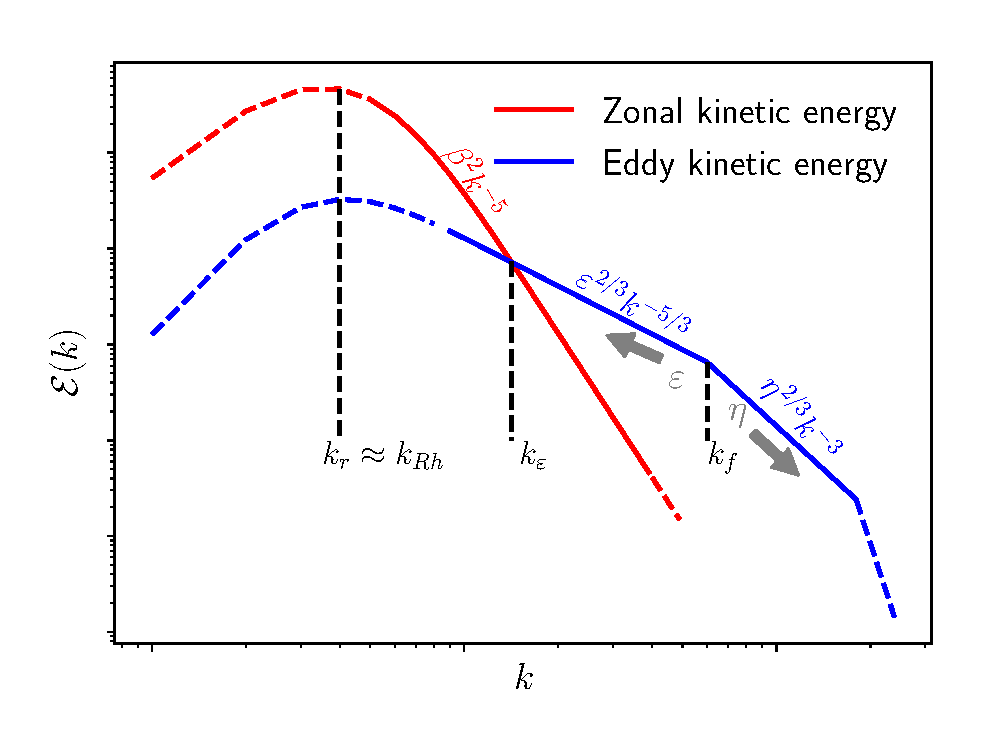
\includegraphics[width=4in]{EKE_ZKE_spectra_illustrate}\caption{Schematic illustration of kinetic energy spectrum in zonal modes (red
line) and eddies (blue) for the zonostrophic turbulence regime. Zonal
and eddy kinetic energy spectra intersect at the crossover wavenumber $k_{\varepsilon}$,
which is thought to be the boundary between near-isotropic turbulence and Rossby
waves. Inverse cascade is halted by friction at $k_{r}$, which is
close to the Rhines wavenumber $k_{Rh}$. The forcing is narrowly
centered at $k_{f}$.}
\label{EKE_KE_spectra_illustrate}
\end{center}
\end{figure}


\begin{figure}
\begin{center}
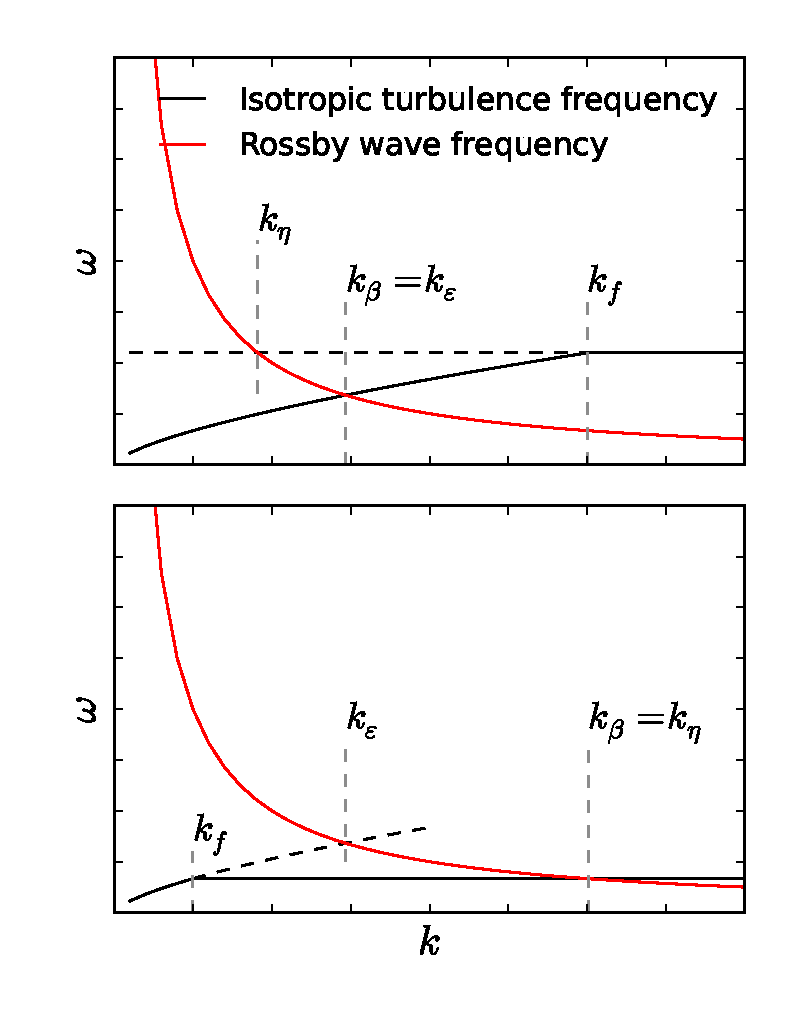
\includegraphics[width=4in]{crossover_scale_illustrate}\caption{Schematic illustration of isotropic turbulence frequency $\omega_{t}$
(black line) and Rossby wave frequency $|\omega_{\beta}|$ (red line).
$\omega_{t}$ and $|\omega_{\beta}|$ intersect (top) within the
inverse energy cascade range or (bottom) within the direct enstrophy
cascade range. The generalized turbulence-wave crossover wavenumber
$k_{\beta}$ is given by either $k_{\varepsilon}$ or $k_{\eta}$
depending on within which range $\omega_{t}$ and $|\omega_{\beta}|$ intersect.}
\label{crossover_illustrate}
\end{center}
\end{figure}


\begin{figure}
\begin{center}
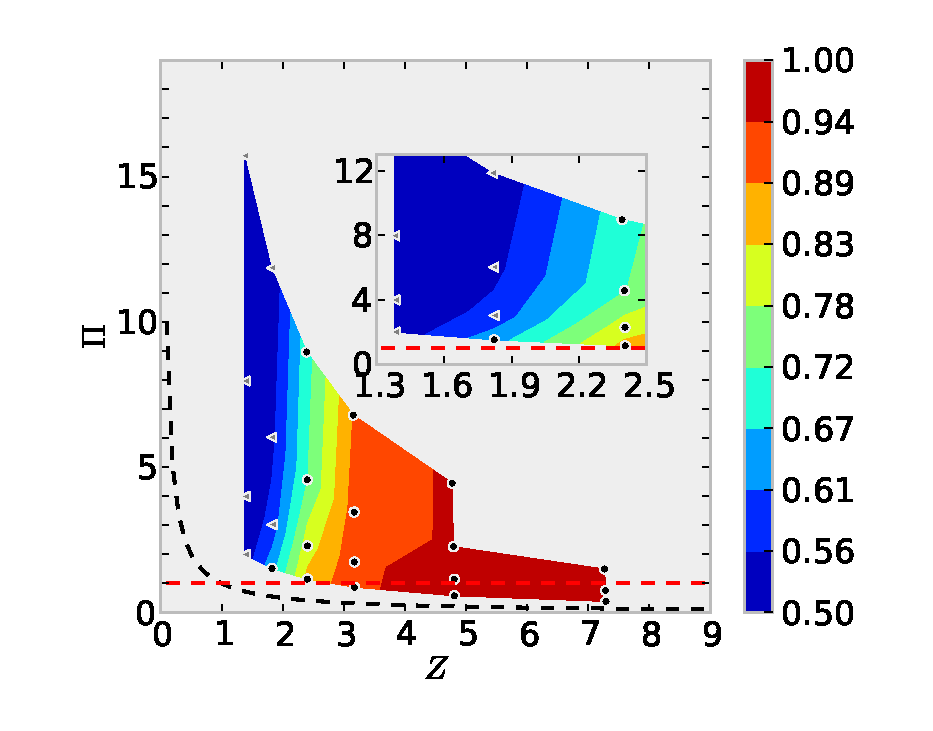
\includegraphics[width=6in]{anisotropic_index}\caption{Anisotropy index defined as $\chi=\langle u^{2}/(u^{2}+v^{2})\rangle$
in the $(Z,\Pi)$ space. The black dots indicate the runs in which
jets have formed, whereas the gray triangles indicate the runs that have
no clear visually identifiable jets. The inset is a zoom-in of the
region $Z\apprle2.5$.}
\label{anisotropic_index}
\end{center}
\end{figure}


\begin{figure}
\begin{center}
\includegraphics[width=6in]{vor_u_drag1024e-4}\caption{Snapshots of relative vorticity (left) and zonal velocity (right)
from $Z=1.8$ runs with $\Pi=$ (top) 1.5, (middle) 6.0, and (bottom)
11.9. The black line in the right panels denote zonal and time mean
zonal wind, with its axis in the bottom right subplot.}
\label{vor_u_snapshot_drag1024e-4}
\end{center}
\end{figure}


\begin{figure}
\begin{center}
\includegraphics[width=6in]{vor_u_drag256e-4}\caption{Snapshots of relative vorticity (left) and zonal velocity (right)
from $Z=2.4$ runs with $\Pi=$ (top) 1.1, (middle) 2.3, and (bottom)
9.0. The black line in the right panels denote zonal and time mean
zonal wind, with its axis in the bottom right subplot.}
\label{vor_u_snapshot_drag256e-4}
\end{center}
\end{figure}


\begin{figure}
\begin{center}
\includegraphics[width=6in]{vor_u_drag8e-4}\caption{Snapshots of relative vorticity (left) and zonal velocity (right)
from $Z=4.8$ runs with $\Pi=$ (top) 0.6, (middle) 1.1, and (bottom)
4.5. The black line in the right panels denote zonal and time mean
zonal wind, with its axis in the bottom right subplot.}
\label{vor_u_snapshot_drag8e-4}
\end{center}
\end{figure}


\begin{figure}
\begin{center}
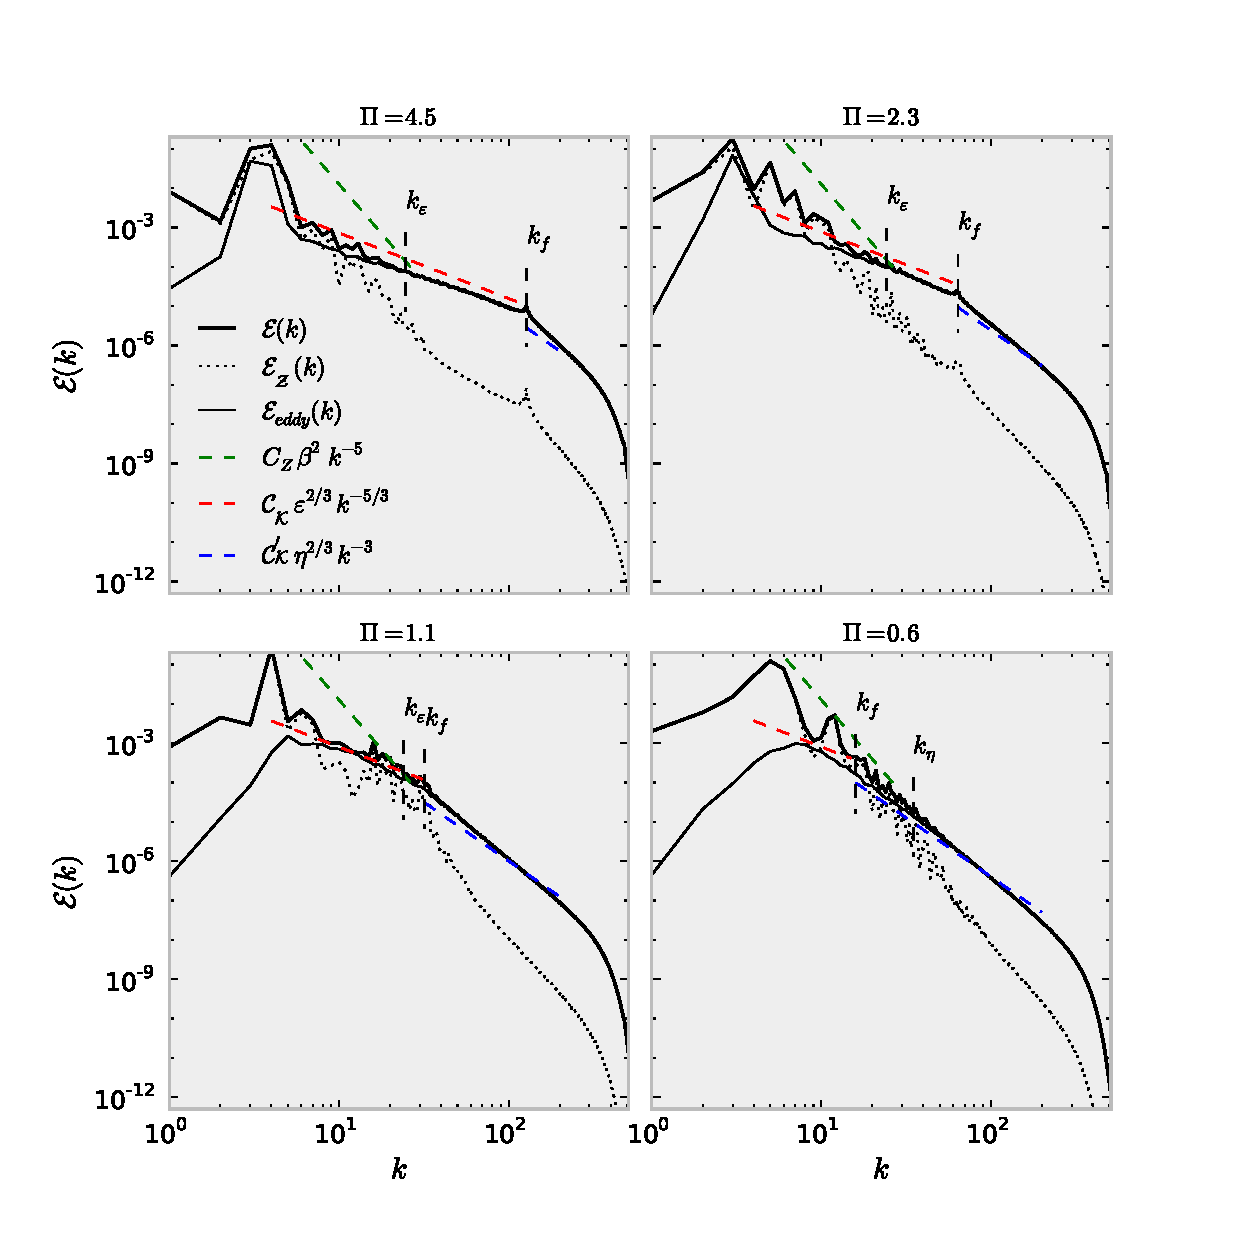
\includegraphics[width=6in]{E_ZKE_EKE_spectra_drag8e-4}\caption{The energy spectra of the total flow $\mathcal{E}(k)$ (thick solid
black line), eddies $\mathcal{E}_{eddy}(k)$ (thin solid black line)
and the zonal flow $\mathcal{E}_{\mathcal{Z}}(k)$ (dotted black line)
from simulations with $Z=4.8$ and various values of $\Pi$ varying
from 0.6 to 4.5 as indicated above the plots. The theoretical spectra
in energy and enstrophy cascade ranges are shown in red and blue dashed
lines respectively. The universal energy spectrum of the zonal modes
with $-5$ slope for zonostrophic turbulence regime is shown in green
dashed line.}
\label{E_EKE_ZKE_spectrum_drag8e-4}
\end{center}
\end{figure}


\begin{figure}
\begin{center}
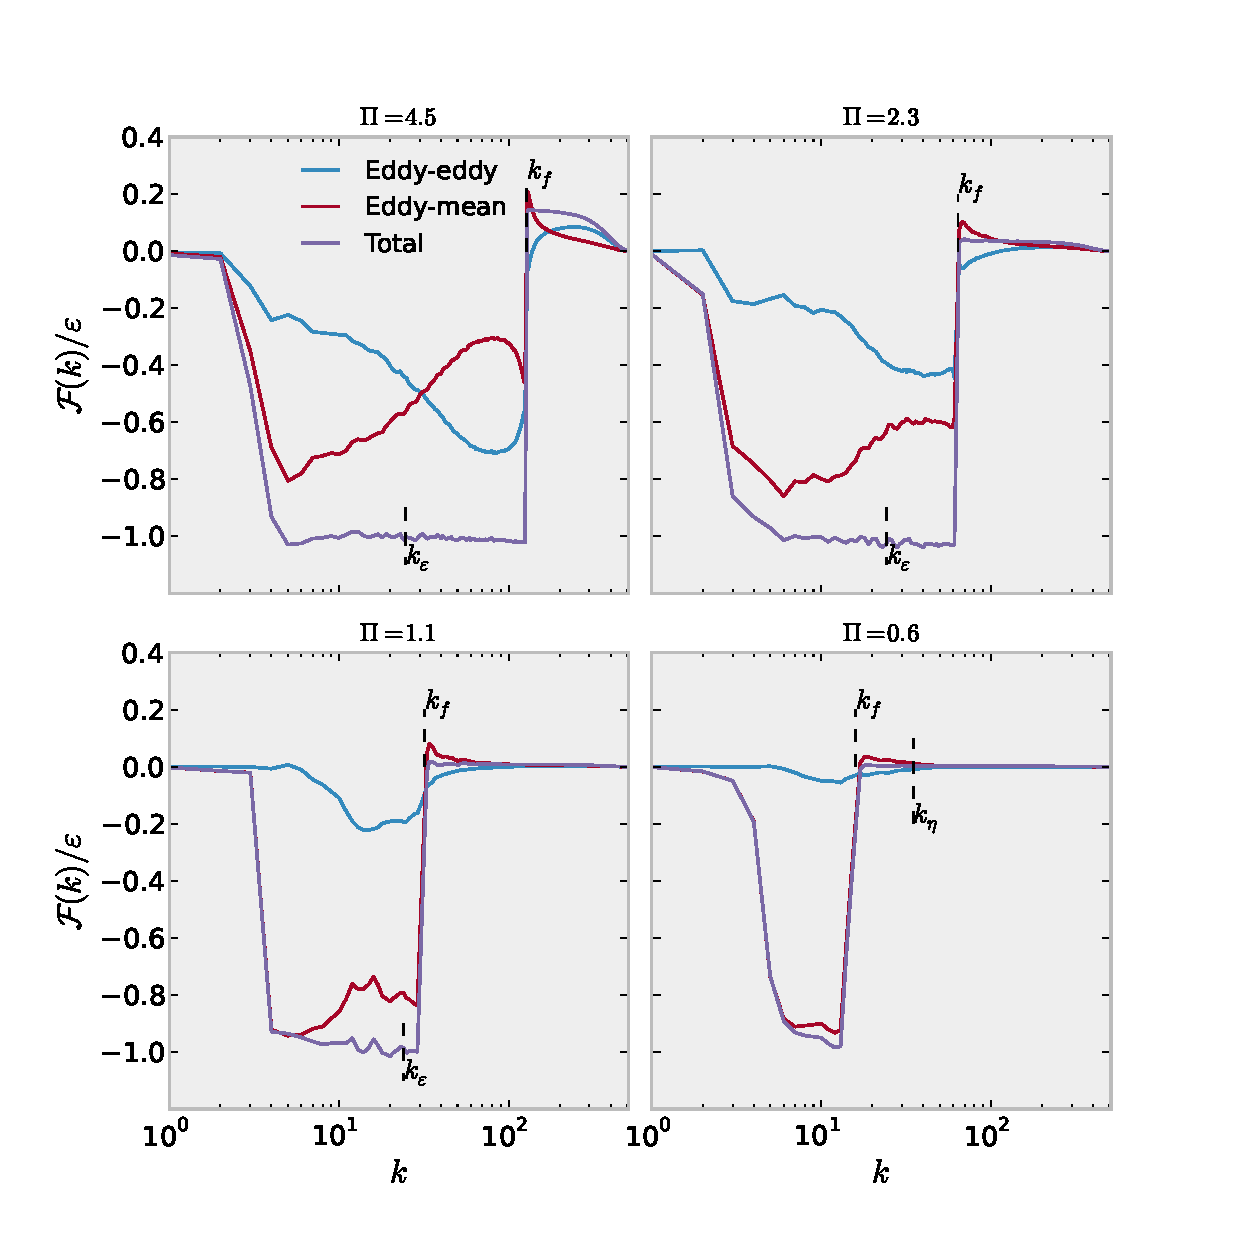
\includegraphics[width=6in]{NLflux_drag8e-4}\caption{Energy flux across wavenumber $k$ for simulations with $Z=4.8$ and
various values of $\Pi$. Energy flux of the total flow $F(k)$ is
the purple line, that of the eddy-eddy interactions $F_{EE}(k)$ is
the blue line, and that of the eddy/mean-flow interactions is the
red line.}
\label{energy_flux_drag8e-4}
\end{center}
\end{figure}


\begin{figure}
\begin{center}
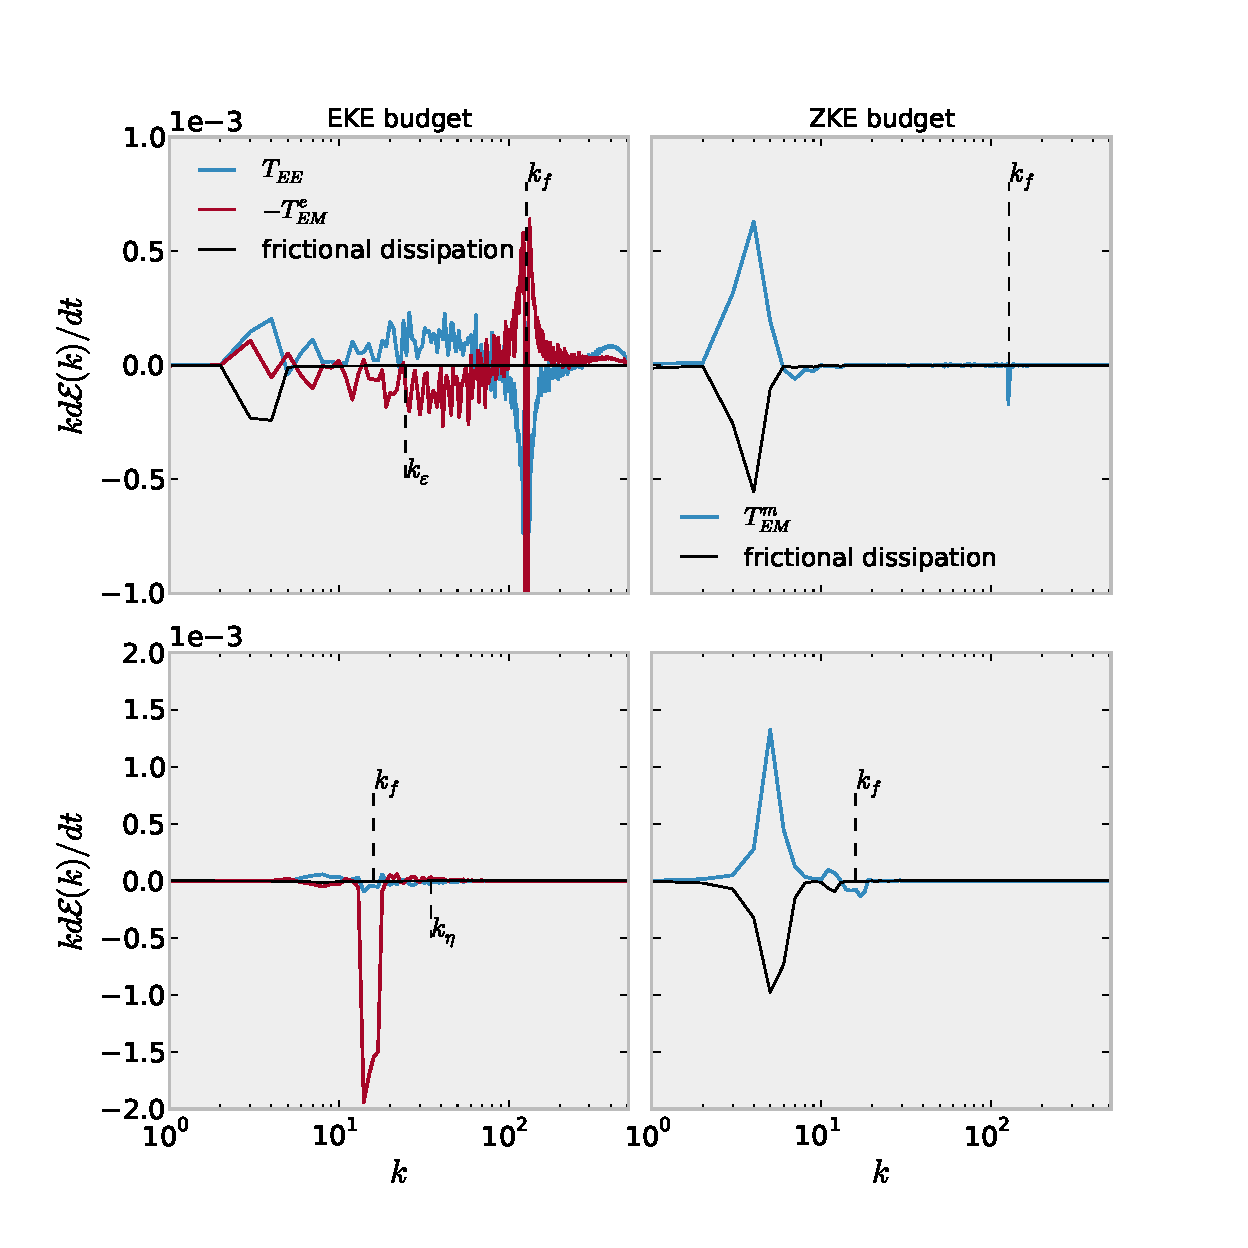
\includegraphics[width=6in]{EKE_ZKE_budget_drag8e-4}\caption{Spectral EKE and ZKE budgets for simulations with $Z=4.8$ and $\Pi=$(top)
4.5 and (bottom) 0.6. The formulation for these budgets are given
in (\ref{eq:EKE_spec_psi}) and (\ref{eq:spectral_ZKE_budget}).}
\label{EKE_ZKE_spectral_budget_drag8e-4}
\end{center}
\end{figure}

\begin{figure}
\begin{center}
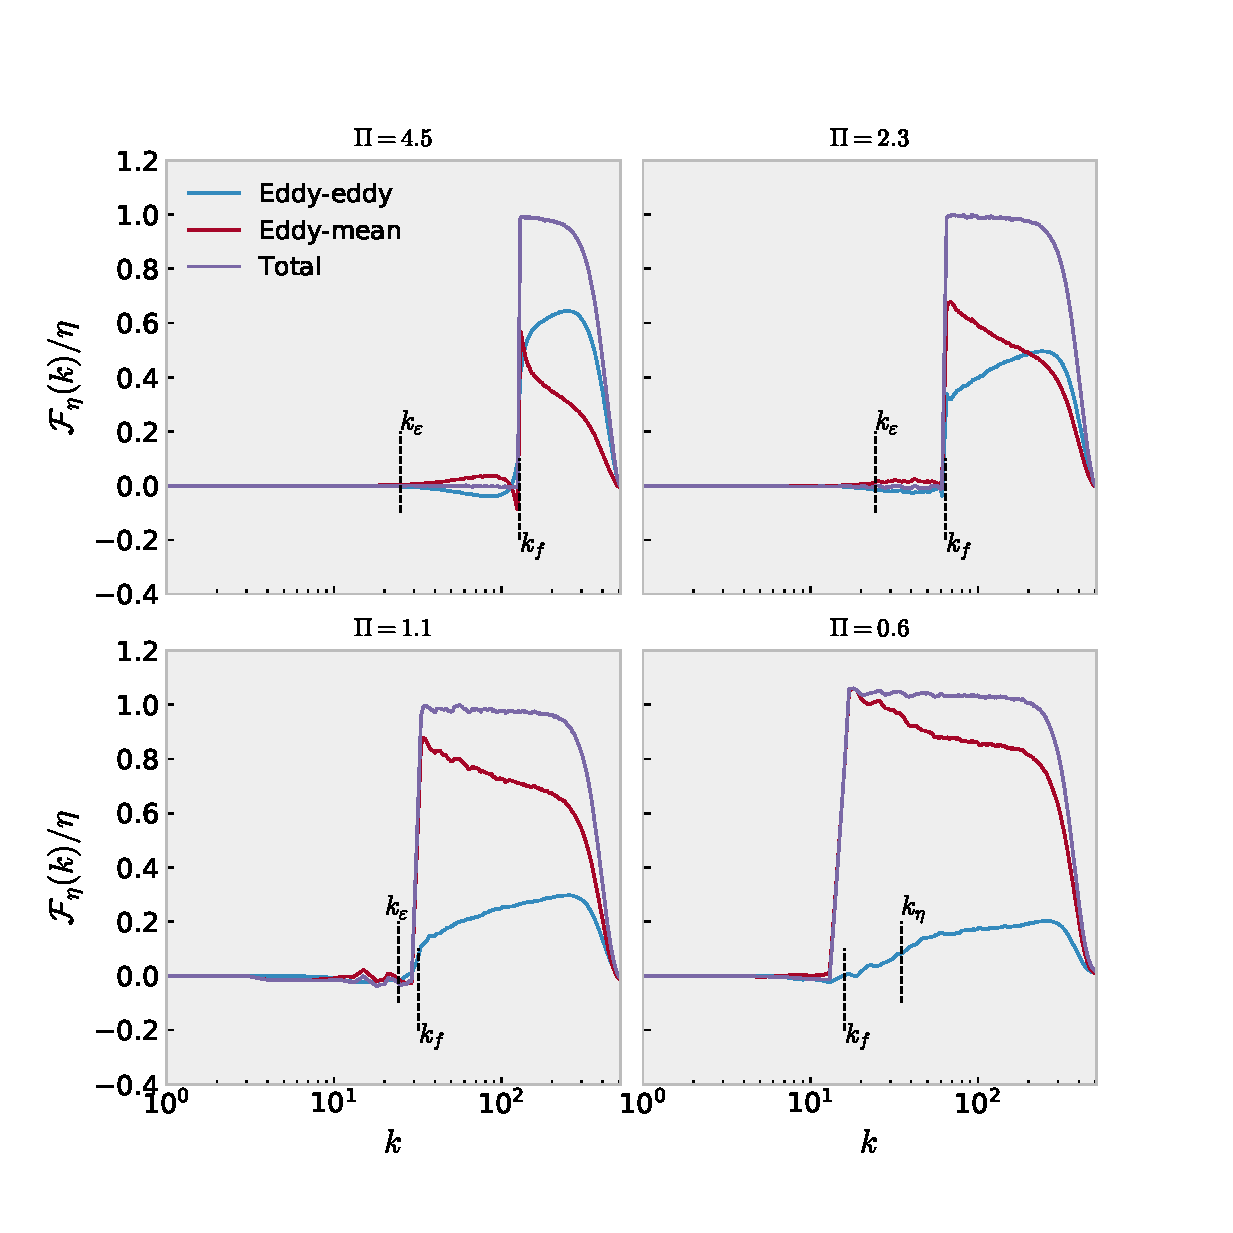
\includegraphics[width=6in]{enstrophy_flux_drag8e-4}\caption{Similar to Fig. (\ref{energy_flux_drag8e-4}) but for enstrophy flux.}
\label{enstrophy_flux_drag8e-4}
\end{center}
\end{figure}


\begin{figure}
\begin{center}
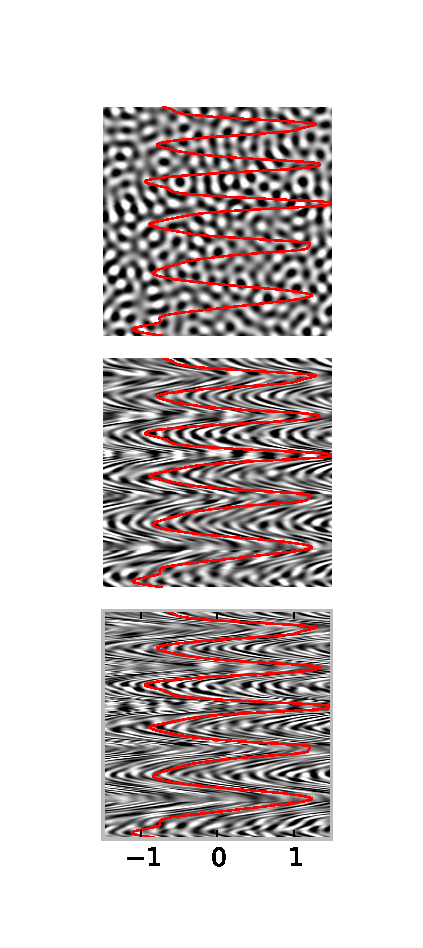
\includegraphics[width=3in]{eddy_vorticity_evolution}\caption{Snapshots of eddy relative vorticity at time $t=0$ (top), 0.78 (middle)
and 1.56 (bottom) from an initial-value run. The red lines denote
the zonal mean zonal wind, with its axis in the bottom subplot. The
parameters for this simulation is the same as $Z=4.8$ but without
forcing and friction. The initial condition is the time and zonal
mean flow from the simulation with $Z=4.8$ and $\Pi=0.6$ run with a
small-amplitude eddy perturbation, which is shown as eddy vorticity
field at $t=0$.}
\label{initial_value_run}
\end{center}
\end{figure}


\begin{figure}
\begin{center}
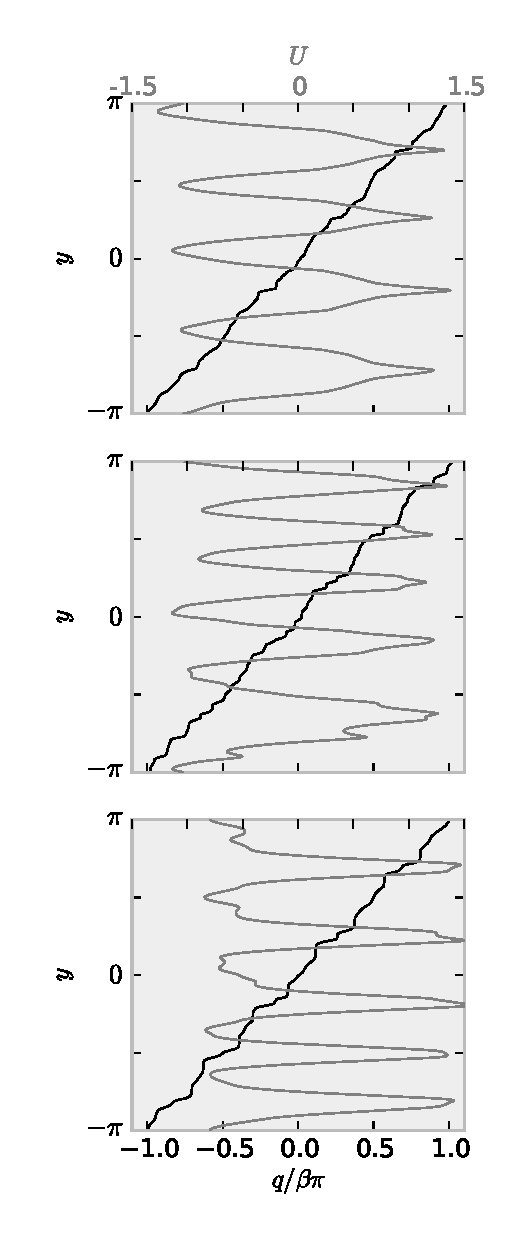
\includegraphics[width=3in]{PV_vs_y}
\caption{Zonal and time mean potential vorticity $\overline{q}$ (black line)
and zonal velocity $\overline{u}$ (gray line) from simulations with
$Z=7.3$ and $\Pi=$(top) 1.5, (middle) 0.76, and (bottom) 0.4. The
potential vorticity profile at equivalent latitude is almost indistinguishable
from $\overline{q}$, so it is not shown.}
\label{PV_vs_y_drag1e-4}
\end{center}
\end{figure}

\begin{figure}
\begin{center}
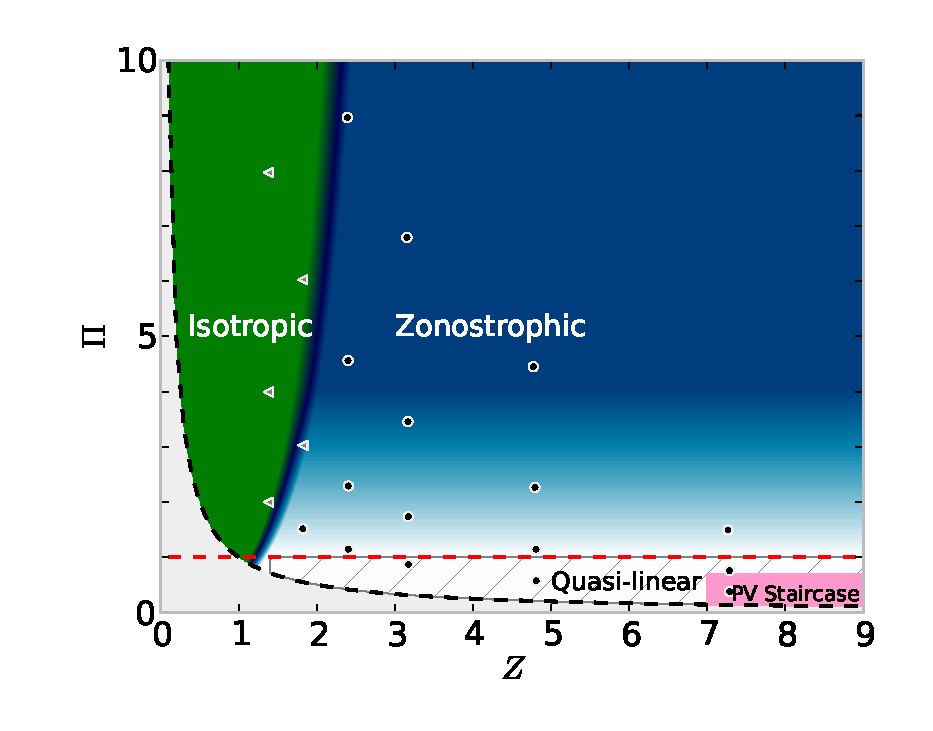
\includegraphics[width=4in]{regime_illustration}\caption{Chart of turbulence regimes in $(Z,\Pi)$ space.}
\label{regime_illustration}
\end{center}
\end{figure}

\end{document}
